\documentclass[1p]{elsarticle_modified}
%\bibliographystyle{elsarticle-num}

%\usepackage[colorlinks]{hyperref}
%\usepackage{abbrmath_seonhwa} %\Abb, \Ascr, \Acal ,\Abf, \Afrak
\usepackage{amsfonts}
\usepackage{amssymb}
\usepackage{amsmath}
\usepackage{amsthm}
\usepackage{scalefnt}
\usepackage{amsbsy}
\usepackage{kotex}
\usepackage{caption}
\usepackage{subfig}
\usepackage{color}
\usepackage{graphicx}
\usepackage{xcolor} %% white, black, red, green, blue, cyan, magenta, yellow
\usepackage{float}
\usepackage{setspace}
\usepackage{hyperref}

\usepackage{tikz}
\usetikzlibrary{arrows}

\usepackage{multirow}
\usepackage{array} % fixed length table
\usepackage{hhline}

%%%%%%%%%%%%%%%%%%%%%
\makeatletter
\renewcommand*\env@matrix[1][\arraystretch]{%
	\edef\arraystretch{#1}%
	\hskip -\arraycolsep
	\let\@ifnextchar\new@ifnextchar
	\array{*\c@MaxMatrixCols c}}
\makeatother %https://tex.stackexchange.com/questions/14071/how-can-i-increase-the-line-spacing-in-a-matrix
%%%%%%%%%%%%%%%

\usepackage[normalem]{ulem}

\newcommand{\msout}[1]{\ifmmode\text{\sout{\ensuremath{#1}}}\else\sout{#1}\fi}
%SOURCE: \msout is \stkout macro in https://tex.stackexchange.com/questions/20609/strikeout-in-math-mode

\newcommand{\cancel}[1]{
	\ifmmode
	{\color{red}\msout{#1}}
	\else
	{\color{red}\sout{#1}}
	\fi
}

\newcommand{\add}[1]{
	{\color{blue}\uwave{#1}}
}

\newcommand{\replace}[2]{
	\ifmmode
	{\color{red}\msout{#1}}{\color{blue}\uwave{#2}}
	\else
	{\color{red}\sout{#1}}{\color{blue}\uwave{#2}}
	\fi
}

\newcommand{\Sol}{\mathcal{S}} %segment
\newcommand{\D}{D} %diagram
\newcommand{\A}{\mathcal{A}} %arc


%%%%%%%%%%%%%%%%%%%%%%%%%%%%%5 test

\def\sl{\operatorname{\textup{SL}}(2,\Cbb)}
\def\psl{\operatorname{\textup{PSL}}(2,\Cbb)}
\def\quan{\mkern 1mu \triangleright \mkern 1mu}

\theoremstyle{definition}
\newtheorem{thm}{Theorem}[section]
\newtheorem{prop}[thm]{Proposition}
\newtheorem{lem}[thm]{Lemma}
\newtheorem{ques}[thm]{Question}
\newtheorem{cor}[thm]{Corollary}
\newtheorem{defn}[thm]{Definition}
\newtheorem{exam}[thm]{Example}
\newtheorem{rmk}[thm]{Remark}
\newtheorem{alg}[thm]{Algorithm}

\newcommand{\I}{\sqrt{-1}}
\begin{document}

%\begin{frontmatter}
%
%\title{Boundary parabolic representations of knots up to 8 crossings}
%
%%% Group authors per affiliation:
%\author{Yunhi Cho} 
%\address{Department of Mathematics, University of Seoul, Seoul, Korea}
%\ead{yhcho@uos.ac.kr}
%
%
%\author{Seonhwa Kim} %\fnref{s_kim}}
%\address{Center for Geometry and Physics, Institute for Basic Science, Pohang, 37673, Korea}
%\ead{ryeona17@ibs.re.kr}
%
%\author{Hyuk Kim}
%\address{Department of Mathematical Sciences, Seoul National University, Seoul 08826, Korea}
%\ead{hyukkim@snu.ac.kr}
%
%\author{Seokbeom Yoon}
%\address{Department of Mathematical Sciences, Seoul National University, Seoul, 08826,  Korea}
%\ead{sbyoon15@snu.ac.kr}
%
%\begin{abstract}
%We find all boundary parabolic representation of knots up to 8 crossings.
%
%\end{abstract}
%\begin{keyword}
%    \MSC[2010] 57M25 
%\end{keyword}
%
%\end{frontmatter}

%\linenumbers
%\tableofcontents
%
\newcommand\colored[1]{\textcolor{white}{\rule[-0.35ex]{0.8em}{1.4ex}}\kern-0.8em\color{red} #1}%
%\newcommand\colored[1]{\textcolor{white}{ #1}\kern-2.17ex	\textcolor{white}{ #1}\kern-1.81ex	\textcolor{white}{ #1}\kern-2.15ex\color{red}#1	}

{\Large $\underline{11a_{158}~(K11a_{158})}$}

\setlength{\tabcolsep}{10pt}
\renewcommand{\arraystretch}{1.6}
\vspace{1cm}\begin{tabular}{m{100pt}>{\centering\arraybackslash}m{274pt}}
\multirow{5}{120pt}{
	\centering
	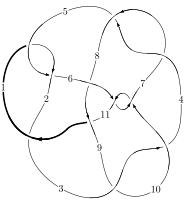
\includegraphics[width=112pt]{../../../GIT/diagram.site/Diagrams/png/407_11a_158.png}\\
\ \ \ A knot diagram\footnotemark}&
\allowdisplaybreaks
\textbf{Linearized knot diagam} \\
\cline{2-2}
 &
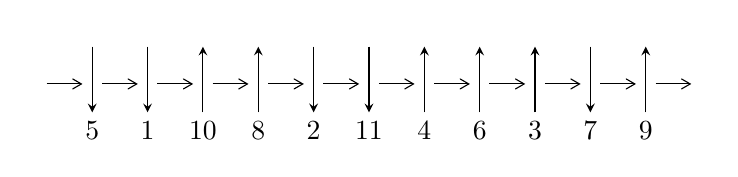
\begin{tikzpicture}[x=20pt, y=17pt]
	% nodes
	\node (C0) at (0, 0) {};
	\node (C1) at (1, 0) {};
	\node (C1U) at (1, +1) {};
	\node (C1D) at (1, -1) {5};

	\node (C2) at (2, 0) {};
	\node (C2U) at (2, +1) {};
	\node (C2D) at (2, -1) {1};

	\node (C3) at (3, 0) {};
	\node (C3U) at (3, +1) {};
	\node (C3D) at (3, -1) {10};

	\node (C4) at (4, 0) {};
	\node (C4U) at (4, +1) {};
	\node (C4D) at (4, -1) {8};

	\node (C5) at (5, 0) {};
	\node (C5U) at (5, +1) {};
	\node (C5D) at (5, -1) {2};

	\node (C6) at (6, 0) {};
	\node (C6U) at (6, +1) {};
	\node (C6D) at (6, -1) {11};

	\node (C7) at (7, 0) {};
	\node (C7U) at (7, +1) {};
	\node (C7D) at (7, -1) {4};

	\node (C8) at (8, 0) {};
	\node (C8U) at (8, +1) {};
	\node (C8D) at (8, -1) {6};

	\node (C9) at (9, 0) {};
	\node (C9U) at (9, +1) {};
	\node (C9D) at (9, -1) {3};

	\node (C10) at (10, 0) {};
	\node (C10U) at (10, +1) {};
	\node (C10D) at (10, -1) {7};

	\node (C11) at (11, 0) {};
	\node (C11U) at (11, +1) {};
	\node (C11D) at (11, -1) {9};
	\node (C12) at (12, 0) {};

	% arrows
	\draw[->,>={angle 60}]
	(C0) edge (C1) (C1) edge (C2) (C2) edge (C3) (C3) edge (C4) (C4) edge (C5) (C5) edge (C6) (C6) edge (C7) (C7) edge (C8) (C8) edge (C9) (C9) edge (C10) (C10) edge (C11) (C11) edge (C12) ;	\draw[->,>=stealth]
	(C1U) edge (C1D) (C2U) edge (C2D) (C3D) edge (C3U) (C4D) edge (C4U) (C5U) edge (C5D) (C6U) edge (C6D) (C7D) edge (C7U) (C8D) edge (C8U) (C9D) edge (C9U) (C10U) edge (C10D) (C11D) edge (C11U) ;
	\end{tikzpicture} \\
\hhline{~~} \\& 
\textbf{Solving Sequence} \\ \cline{2-2} 
 &
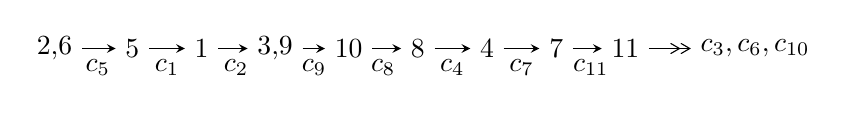
\begin{tikzpicture}[x=25pt, y=7pt]
	% node
	\node (A0) at (-1/8, 0) {2,6};
	\node (A1) at (1, 0) {5};
	\node (A2) at (2, 0) {1};
	\node (A3) at (49/16, 0) {3,9};
	\node (A4) at (33/8, 0) {10};
	\node (A5) at (41/8, 0) {8};
	\node (A6) at (49/8, 0) {4};
	\node (A7) at (57/8, 0) {7};
	\node (A8) at (65/8, 0) {11};
	\node (C1) at (1/2, -1) {$c_{5}$};
	\node (C2) at (3/2, -1) {$c_{1}$};
	\node (C3) at (5/2, -1) {$c_{2}$};
	\node (C4) at (29/8, -1) {$c_{9}$};
	\node (C5) at (37/8, -1) {$c_{8}$};
	\node (C6) at (45/8, -1) {$c_{4}$};
	\node (C7) at (53/8, -1) {$c_{7}$};
	\node (C8) at (61/8, -1) {$c_{11}$};
	\node (A9) at (10, 0) {$c_{3},c_{6},c_{10}$};

	% edge
	\draw[->,>=stealth]	
	(A0) edge (A1) (A1) edge (A2) (A2) edge (A3) (A3) edge (A4) (A4) edge (A5) (A5) edge (A6) (A6) edge (A7) (A7) edge (A8) ;
	\draw[->>,>={angle 60}]	
	(A8) edge (A9);
\end{tikzpicture} \\ 

\end{tabular} \\

\footnotetext{
The image of knot diagram is generated by the software ``\textbf{Draw programme}" developed by Andrew Bartholomew(\url{http://www.layer8.co.uk/maths/draw/index.htm\#Running-draw}), where we modified some parts for our purpose(\url{https://github.com/CATsTAILs/LinksPainter}).
}\phantom \\ \newline 
\centering \textbf{Ideals for irreducible components\footnotemark of $X_{\text{par}}$} 
 
\begin{align*}
I^u_{1}&=\langle 
23 u^{27}+131 u^{26}+\cdots+4 b+148,\;273 u^{27}+2147 u^{26}+\cdots+8 a-1460,\;u^{28}+9 u^{27}+\cdots-52 u-8\rangle \\
I^u_{2}&=\langle 
5.27001\times10^{16} a^{5} u^{7}-2.11866\times10^{16} a^{4} u^{7}+\cdots-8.58870\times10^{16} a+2.09109\times10^{17},\\
\phantom{I^u_{2}}&\phantom{= \langle  }u^7 a^5-7 u^7 a^4+\cdots-92 a-320,\;u^8- u^7- u^6+2 u^5+u^4-2 u^3+2 u-1\rangle \\
I^u_{3}&=\langle 
-2 u^{16}+4 u^{15}+\cdots+b+3,\;-4 u^{16}+7 u^{15}+\cdots+a+11,\;u^{17}-2 u^{16}+\cdots-4 u+1\rangle \\
\\
\end{align*}
\raggedright * 3 irreducible components of $\dim_{\mathbb{C}}=0$, with total 93 representations.\\
\footnotetext{All coefficients of polynomials are rational numbers. But the coefficients are sometimes approximated in decimal forms when there is not enough margin.}
\newpage
\renewcommand{\arraystretch}{1}
\centering \section*{I. $I^u_{1}= \langle 23 u^{27}+131 u^{26}+\cdots+4 b+148,\;273 u^{27}+2147 u^{26}+\cdots+8 a-1460,\;u^{28}+9 u^{27}+\cdots-52 u-8 \rangle$}
\flushleft \textbf{(i) Arc colorings}\\
\begin{tabular}{m{7pt} m{180pt} m{7pt} m{180pt} }
\flushright $a_{2}=$&$\begin{pmatrix}0\\u\end{pmatrix}$ \\
\flushright $a_{6}=$&$\begin{pmatrix}1\\0\end{pmatrix}$ \\
\flushright $a_{5}=$&$\begin{pmatrix}1\\- u^2\end{pmatrix}$ \\
\flushright $a_{1}=$&$\begin{pmatrix}u\\- u^3+u\end{pmatrix}$ \\
\flushright $a_{3}=$&$\begin{pmatrix}- u^3\\u^5- u^3+u\end{pmatrix}$ \\
\flushright $a_{9}=$&$\begin{pmatrix}-34.1250 u^{27}-268.375 u^{26}+\cdots+1118.25 u+182.500\\-\frac{23}{4} u^{27}-\frac{131}{4} u^{26}+\cdots-150 u-37\end{pmatrix}$ \\
\flushright $a_{10}=$&$\begin{pmatrix}-7.12500 u^{27}-50.3750 u^{26}+\cdots+178.250 u+30.5000\\\frac{21}{4} u^{27}+\frac{173}{4} u^{26}+\cdots-236 u-43\end{pmatrix}$ \\
\flushright $a_{8}=$&$\begin{pmatrix}-28.3750 u^{27}-235.625 u^{26}+\cdots+1268.25 u+219.500\\-\frac{23}{4} u^{27}-\frac{131}{4} u^{26}+\cdots-150 u-37\end{pmatrix}$ \\
\flushright $a_{4}=$&$\begin{pmatrix}\frac{35}{8} u^{27}+\frac{305}{8} u^{26}+\cdots-\frac{923}{4} u-40\\\frac{9}{4} u^{27}+\frac{55}{4} u^{26}+\cdots+\frac{75}{2} u+9\end{pmatrix}$ \\
\flushright $a_{7}=$&$\begin{pmatrix}-\frac{127}{8} u^{27}-\frac{1007}{8} u^{26}+\cdots+\frac{1119}{2} u+92\\2 u^{27}+\frac{31}{2} u^{26}+\cdots-\frac{161}{2} u-15\end{pmatrix}$ \\
\flushright $a_{11}=$&$\begin{pmatrix}-\frac{77}{8} u^{27}-\frac{671}{8} u^{26}+\cdots+\frac{2185}{4} u+95\\-\frac{37}{4} u^{27}-\frac{299}{4} u^{26}+\cdots+\frac{681}{2} u+55\end{pmatrix}$\\ \flushright $a_{11}=$&$\begin{pmatrix}-\frac{77}{8} u^{27}-\frac{671}{8} u^{26}+\cdots+\frac{2185}{4} u+95\\-\frac{37}{4} u^{27}-\frac{299}{4} u^{26}+\cdots+\frac{681}{2} u+55\end{pmatrix}$\\&\end{tabular}
\flushleft \textbf{(ii) Obstruction class $= -1$}\\~\\
\flushleft \textbf{(iii) Cusp Shapes $= 72 u^{27}+580 u^{26}+1879 u^{25}+2101 u^{24}-4589 u^{23}-20304 u^{22}-26684 u^{21}+10295 u^{20}+87084 u^{19}+117201 u^{18}+4207 u^{17}-196492 u^{16}-261463 u^{15}-51078 u^{14}+257673 u^{13}+330937 u^{12}+85897 u^{11}-201772 u^{10}-247215 u^9-76609 u^8+80609 u^7+98024 u^6+35254 u^5-10933 u^4-17557 u^3-8954 u^2-2662 u-434$}\\~\\
\newpage\renewcommand{\arraystretch}{1}
\flushleft \textbf{(iv) u-Polynomials at the component}\newline \\
\begin{tabular}{m{50pt}|m{274pt}}
Crossings & \hspace{64pt}u-Polynomials at each crossing \\
\hline $$\begin{aligned}c_{1},c_{5}\end{aligned}$$&$\begin{aligned}
&u^{28}+9 u^{27}+\cdots-52 u-8
\end{aligned}$\\
\hline $$\begin{aligned}c_{2}\end{aligned}$$&$\begin{aligned}
&u^{28}+13 u^{27}+\cdots-304 u+64
\end{aligned}$\\
\hline $$\begin{aligned}c_{3},c_{4},c_{7}\\c_{9}\end{aligned}$$&$\begin{aligned}
&u^{28}- u^{27}+\cdots-3 u+1
\end{aligned}$\\
\hline $$\begin{aligned}c_{6},c_{10}\end{aligned}$$&$\begin{aligned}
&u^{28}+18 u^{27}+\cdots-3328 u-256
\end{aligned}$\\
\hline $$\begin{aligned}c_{8},c_{11}\end{aligned}$$&$\begin{aligned}
&u^{28}+2 u^{27}+\cdots-8 u+1
\end{aligned}$\\
\hline
\end{tabular}\\~\\
\newpage\renewcommand{\arraystretch}{1}
\flushleft \textbf{(v) Riley Polynomials at the component}\newline \\
\begin{tabular}{m{50pt}|m{274pt}}
Crossings & \hspace{64pt}Riley Polynomials at each crossing \\
\hline $$\begin{aligned}c_{1},c_{5}\end{aligned}$$&$\begin{aligned}
&y^{28}-13 y^{27}+\cdots+304 y+64
\end{aligned}$\\
\hline $$\begin{aligned}c_{2}\end{aligned}$$&$\begin{aligned}
&y^{28}+7 y^{27}+\cdots-204032 y+4096
\end{aligned}$\\
\hline $$\begin{aligned}c_{3},c_{4},c_{7}\\c_{9}\end{aligned}$$&$\begin{aligned}
&y^{28}-27 y^{27}+\cdots-3 y+1
\end{aligned}$\\
\hline $$\begin{aligned}c_{6},c_{10}\end{aligned}$$&$\begin{aligned}
&y^{28}+14 y^{27}+\cdots-303104 y^2+65536
\end{aligned}$\\
\hline $$\begin{aligned}c_{8},c_{11}\end{aligned}$$&$\begin{aligned}
&y^{28}-12 y^{27}+\cdots-66 y+1
\end{aligned}$\\
\hline
\end{tabular}\\~\\
\newpage\flushleft \textbf{(vi) Complex Volumes and Cusp Shapes}
$$\begin{array}{c|c|c}  
\text{Solutions to }I^u_{1}& \I (\text{vol} + \sqrt{-1}CS) & \text{Cusp shape}\\
 \hline 
\begin{aligned}
u &= \phantom{-}0.993549 + 0.292986 I \\
a &= -0.209833 - 0.434545 I \\
b &= \phantom{-}0.017296 + 1.007040 I\end{aligned}
 & -2.36961 - 3.39893 I & -1.55352 + 8.34822 I \\ \hline\begin{aligned}
u &= \phantom{-}0.993549 - 0.292986 I \\
a &= -0.209833 + 0.434545 I \\
b &= \phantom{-}0.017296 - 1.007040 I\end{aligned}
 & -2.36961 + 3.39893 I & -1.55352 - 8.34822 I \\ \hline\begin{aligned}
u &= -0.745676 + 0.599578 I \\
a &= -1.08882 + 1.35793 I \\
b &= -0.997965 + 0.424920 I\end{aligned}
 & \phantom{-}1.93199 - 0.88418 I & \phantom{-}2.93120 + 0.94418 I \\ \hline\begin{aligned}
u &= -0.745676 - 0.599578 I \\
a &= -1.08882 - 1.35793 I \\
b &= -0.997965 - 0.424920 I\end{aligned}
 & \phantom{-}1.93199 + 0.88418 I & \phantom{-}2.93120 - 0.94418 I \\ \hline\begin{aligned}
u &= -0.910751 + 0.513446 I \\
a &= \phantom{-}1.303570 - 0.508382 I \\
b &= \phantom{-}0.664049 + 0.374496 I\end{aligned}
 & -1.19975 + 1.98781 I & -3.01378 - 1.84233 I \\ \hline\begin{aligned}
u &= -0.910751 - 0.513446 I \\
a &= \phantom{-}1.303570 + 0.508382 I \\
b &= \phantom{-}0.664049 - 0.374496 I\end{aligned}
 & -1.19975 - 1.98781 I & -3.01378 + 1.84233 I \\ \hline\begin{aligned}
u &= -0.924272 + 0.615006 I \\
a &= -1.94919 + 0.56217 I \\
b &= -1.167050 - 0.765226 I\end{aligned}
 & \phantom{-}1.38789 + 5.70099 I & \phantom{-}1.78458 - 5.41589 I \\ \hline\begin{aligned}
u &= -0.924272 - 0.615006 I \\
a &= -1.94919 - 0.56217 I \\
b &= -1.167050 + 0.765226 I\end{aligned}
 & \phantom{-}1.38789 - 5.70099 I & \phantom{-}1.78458 + 5.41589 I \\ \hline\begin{aligned}
u &= -0.582336 + 0.951705 I \\
a &= \phantom{-}1.14682 - 0.86852 I \\
b &= \phantom{-}1.45377 - 0.81817 I\end{aligned}
 & \phantom{-}13.5292 - 10.0747 I & \phantom{-}8.45933 + 4.17008 I \\ \hline\begin{aligned}
u &= -0.582336 - 0.951705 I \\
a &= \phantom{-}1.14682 + 0.86852 I \\
b &= \phantom{-}1.45377 + 0.81817 I\end{aligned}
 & \phantom{-}13.5292 + 10.0747 I & \phantom{-}8.45933 - 4.17008 I\\
 \hline 
 \end{array}$$\newpage$$\begin{array}{c|c|c}  
\text{Solutions to }I^u_{1}& \I (\text{vol} + \sqrt{-1}CS) & \text{Cusp shape}\\
 \hline 
\begin{aligned}
u &= -0.443366 + 1.056140 I \\
a &= \phantom{-}0.787450 + 0.068648 I \\
b &= \phantom{-}1.080890 - 0.000686 I\end{aligned}
 & \phantom{-}12.38150 + 4.38665 I & \phantom{-}10.97973 - 3.34546 I \\ \hline\begin{aligned}
u &= -0.443366 - 1.056140 I \\
a &= \phantom{-}0.787450 - 0.068648 I \\
b &= \phantom{-}1.080890 + 0.000686 I\end{aligned}
 & \phantom{-}12.38150 - 4.38665 I & \phantom{-}10.97973 + 3.34546 I \\ \hline\begin{aligned}
u &= \phantom{-}0.807574 + 0.208228 I \\
a &= \phantom{-}0.576875 + 0.559894 I \\
b &= -0.512192 - 1.107170 I\end{aligned}
 & -1.14045 + 1.47239 I & \phantom{-}6.24854 + 6.39498 I \\ \hline\begin{aligned}
u &= \phantom{-}0.807574 - 0.208228 I \\
a &= \phantom{-}0.576875 - 0.559894 I \\
b &= -0.512192 + 1.107170 I\end{aligned}
 & -1.14045 - 1.47239 I & \phantom{-}6.24854 - 6.39498 I \\ \hline\begin{aligned}
u &= -0.593204 + 1.035470 I \\
a &= -0.760509 + 0.545380 I \\
b &= -1.104210 + 0.569568 I\end{aligned}
 & \phantom{-}7.89930 - 3.44261 I & \phantom{-}8.17074 + 2.94837 I \\ \hline\begin{aligned}
u &= -0.593204 - 1.035470 I \\
a &= -0.760509 - 0.545380 I \\
b &= -1.104210 - 0.569568 I\end{aligned}
 & \phantom{-}7.89930 + 3.44261 I & \phantom{-}8.17074 - 2.94837 I \\ \hline\begin{aligned}
u &= -1.31909\phantom{ +0.000000I} \\
a &= \phantom{-}0.297585\phantom{ +0.000000I} \\
b &= -0.125254\phantom{ +0.000000I}\end{aligned}
 & -3.01060\phantom{ +0.000000I} & -14.4720\phantom{ +0.000000I} \\ \hline\begin{aligned}
u &= -1.106870 + 0.732140 I \\
a &= \phantom{-}1.60551 - 0.89150 I \\
b &= \phantom{-}1.46289 + 1.05428 I\end{aligned}
 & \phantom{-}11.9038 + 16.2350 I & \phantom{-}6.36027 - 8.32086 I \\ \hline\begin{aligned}
u &= -1.106870 - 0.732140 I \\
a &= \phantom{-}1.60551 + 0.89150 I \\
b &= \phantom{-}1.46289 - 1.05428 I\end{aligned}
 & \phantom{-}11.9038 - 16.2350 I & \phantom{-}6.36027 + 8.32086 I \\ \hline\begin{aligned}
u &= \phantom{-}1.320980 + 0.142620 I \\
a &= -0.245968 + 0.237735 I \\
b &= \phantom{-}0.872613 - 0.596296 I\end{aligned}
 & \phantom{-}5.89990 - 8.09391 I & \phantom{-}4.42894 + 6.82969 I\\
 \hline 
 \end{array}$$\newpage$$\begin{array}{c|c|c}  
\text{Solutions to }I^u_{1}& \I (\text{vol} + \sqrt{-1}CS) & \text{Cusp shape}\\
 \hline 
\begin{aligned}
u &= \phantom{-}1.320980 - 0.142620 I \\
a &= -0.245968 - 0.237735 I \\
b &= \phantom{-}0.872613 + 0.596296 I\end{aligned}
 & \phantom{-}5.89990 + 8.09391 I & \phantom{-}4.42894 - 6.82969 I \\ \hline\begin{aligned}
u &= -1.124600 + 0.770804 I \\
a &= -1.196350 + 0.572951 I \\
b &= -1.094850 - 0.891823 I\end{aligned}
 & \phantom{-}6.23596 + 9.95004 I & \phantom{-}5.25531 - 7.03832 I \\ \hline\begin{aligned}
u &= -1.124600 - 0.770804 I \\
a &= -1.196350 - 0.572951 I \\
b &= -1.094850 + 0.891823 I\end{aligned}
 & \phantom{-}6.23596 - 9.95004 I & \phantom{-}5.25531 + 7.03832 I \\ \hline\begin{aligned}
u &= -1.22157 + 0.75184 I \\
a &= \phantom{-}0.498779 - 0.680355 I \\
b &= \phantom{-}0.885139 + 0.340742 I\end{aligned}
 & \phantom{-}10.00870 + 2.13523 I & \phantom{-}9.70507 + 0. I\phantom{ +0.000000I} \\ \hline\begin{aligned}
u &= -1.22157 - 0.75184 I \\
a &= \phantom{-}0.498779 + 0.680355 I \\
b &= \phantom{-}0.885139 - 0.340742 I\end{aligned}
 & \phantom{-}10.00870 - 2.13523 I & \phantom{-}9.70507 + 0. I\phantom{ +0.000000I} \\ \hline\begin{aligned}
u &= \phantom{-}1.55763\phantom{ +0.000000I} \\
a &= \phantom{-}0.154610\phantom{ +0.000000I} \\
b &= -0.615944\phantom{ +0.000000I}\end{aligned}
 & -0.410918\phantom{ +0.000000I} & \phantom{-}16.4090\phantom{ +0.000000I} \\ \hline\begin{aligned}
u &= -0.088743 + 0.380871 I \\
a &= \phantom{-}0.555578 - 1.006500 I \\
b &= -0.189785 - 0.401445 I\end{aligned}
 & \phantom{-}0.217297 + 1.036000 I & \phantom{-}3.27495 - 6.74585 I \\ \hline\begin{aligned}
u &= -0.088743 - 0.380871 I \\
a &= \phantom{-}0.555578 + 1.006500 I \\
b &= -0.189785 + 0.401445 I\end{aligned}
 & \phantom{-}0.217297 - 1.036000 I & \phantom{-}3.27495 + 6.74585 I\\
 \hline 
 \end{array}$$\newpage\newpage\renewcommand{\arraystretch}{1}
\centering \section*{II. $I^u_{2}= \langle 5.27\times10^{16} a^{5} u^{7}-2.12\times10^{16} a^{4} u^{7}+\cdots-8.59\times10^{16} a+2.09\times10^{17},\;u^7 a^5-7 u^7 a^4+\cdots-92 a-320,\;u^8- u^7- u^6+2 u^5+u^4-2 u^3+2 u-1 \rangle$}
\flushleft \textbf{(i) Arc colorings}\\
\begin{tabular}{m{7pt} m{180pt} m{7pt} m{180pt} }
\flushright $a_{2}=$&$\begin{pmatrix}0\\u\end{pmatrix}$ \\
\flushright $a_{6}=$&$\begin{pmatrix}1\\0\end{pmatrix}$ \\
\flushright $a_{5}=$&$\begin{pmatrix}1\\- u^2\end{pmatrix}$ \\
\flushright $a_{1}=$&$\begin{pmatrix}u\\- u^3+u\end{pmatrix}$ \\
\flushright $a_{3}=$&$\begin{pmatrix}- u^3\\u^5- u^3+u\end{pmatrix}$ \\
\flushright $a_{9}=$&$\begin{pmatrix}a\\-0.382668 a^{5} u^{7}+0.153841 a^{4} u^{7}+\cdots+0.623646 a-1.51839\end{pmatrix}$ \\
\flushright $a_{10}=$&$\begin{pmatrix}-0.638309 a^{5} u^{7}+0.178480 a^{4} u^{7}+\cdots+0.861026 a+0.0250433\\0.274885 a^{5} u^{7}+0.113800 a^{4} u^{7}+\cdots+0.225598 a-1.44869\end{pmatrix}$ \\
\flushright $a_{8}=$&$\begin{pmatrix}0.382668 a^{5} u^{7}-0.153841 a^{4} u^{7}+\cdots+0.376354 a+1.51839\\-0.382668 a^{5} u^{7}+0.153841 a^{4} u^{7}+\cdots+0.623646 a-1.51839\end{pmatrix}$ \\
\flushright $a_{4}=$&$\begin{pmatrix}-0.941009 a^{5} u^{7}-0.361240 a^{4} u^{7}+\cdots+0.0598849 a+1.73126\\0.895289 a^{5} u^{7}+0.368189 a^{4} u^{7}+\cdots+0.398274 a+2.83473\end{pmatrix}$ \\
\flushright $a_{7}=$&$\begin{pmatrix}-0.830940 a^{5} u^{7}-0.669583 a^{4} u^{7}+\cdots-0.192170 a+8.12188\\0.629283 a^{5} u^{7}+0.240763 a^{4} u^{7}+\cdots-0.268495 a-0.378118\end{pmatrix}$ \\
\flushright $a_{11}=$&$\begin{pmatrix}-0.517443 a^{5} u^{7}-0.185517 a^{4} u^{7}+\cdots-0.234948 a+3.55145\\0.904169 a^{5} u^{7}+0.354563 a^{4} u^{7}+\cdots-0.0428966 a-0.826810\end{pmatrix}$\\ \flushright $a_{11}=$&$\begin{pmatrix}-0.517443 a^{5} u^{7}-0.185517 a^{4} u^{7}+\cdots-0.234948 a+3.55145\\0.904169 a^{5} u^{7}+0.354563 a^{4} u^{7}+\cdots-0.0428966 a-0.826810\end{pmatrix}$\\&\end{tabular}
\flushleft \textbf{(ii) Obstruction class $= -1$}\\~\\
\flushleft \textbf{(iii) Cusp Shapes $= \frac{151426107279833992}{137717486950419293} u^7 a^5+\frac{62688797470204452}{137717486950419293} u^7 a^4+\cdots+\frac{124275431271284696}{137717486950419293} a-\frac{1073475726019287126}{137717486950419293}$}\\~\\
\newpage\renewcommand{\arraystretch}{1}
\flushleft \textbf{(iv) u-Polynomials at the component}\newline \\
\begin{tabular}{m{50pt}|m{274pt}}
Crossings & \hspace{64pt}u-Polynomials at each crossing \\
\hline $$\begin{aligned}c_{1},c_{5}\end{aligned}$$&$\begin{aligned}
&(u^8- u^7- u^6+2 u^5+u^4-2 u^3+2 u-1)^6
\end{aligned}$\\
\hline $$\begin{aligned}c_{2}\end{aligned}$$&$\begin{aligned}
&(u^8+3 u^7+7 u^6+10 u^5+11 u^4+10 u^3+6 u^2+4 u+1)^6
\end{aligned}$\\
\hline $$\begin{aligned}c_{3},c_{4},c_{7}\\c_{9}\end{aligned}$$&$\begin{aligned}
&u^{48}- u^{47}+\cdots+348 u-701
\end{aligned}$\\
\hline $$\begin{aligned}c_{6},c_{10}\end{aligned}$$&$\begin{aligned}
&(u^3- u^2+2 u-1)^{16}
\end{aligned}$\\
\hline $$\begin{aligned}c_{8},c_{11}\end{aligned}$$&$\begin{aligned}
&u^{48}+9 u^{47}+\cdots+1494 u+1151
\end{aligned}$\\
\hline
\end{tabular}\\~\\
\newpage\renewcommand{\arraystretch}{1}
\flushleft \textbf{(v) Riley Polynomials at the component}\newline \\
\begin{tabular}{m{50pt}|m{274pt}}
Crossings & \hspace{64pt}Riley Polynomials at each crossing \\
\hline $$\begin{aligned}c_{1},c_{5}\end{aligned}$$&$\begin{aligned}
&(y^8-3 y^7+7 y^6-10 y^5+11 y^4-10 y^3+6 y^2-4 y+1)^6
\end{aligned}$\\
\hline $$\begin{aligned}c_{2}\end{aligned}$$&$\begin{aligned}
&(y^8+5 y^7+11 y^6+6 y^5-17 y^4-34 y^3-22 y^2-4 y+1)^6
\end{aligned}$\\
\hline $$\begin{aligned}c_{3},c_{4},c_{7}\\c_{9}\end{aligned}$$&$\begin{aligned}
&y^{48}-45 y^{47}+\cdots+8666632 y+491401
\end{aligned}$\\
\hline $$\begin{aligned}c_{6},c_{10}\end{aligned}$$&$\begin{aligned}
&(y^3+3 y^2+2 y-1)^{16}
\end{aligned}$\\
\hline $$\begin{aligned}c_{8},c_{11}\end{aligned}$$&$\begin{aligned}
&y^{48}-17 y^{47}+\cdots-69505684 y+1324801
\end{aligned}$\\
\hline
\end{tabular}\\~\\
\newpage\flushleft \textbf{(vi) Complex Volumes and Cusp Shapes}
$$\begin{array}{c|c|c}  
\text{Solutions to }I^u_{2}& \I (\text{vol} + \sqrt{-1}CS) & \text{Cusp shape}\\
 \hline 
\begin{aligned}
u &= \phantom{-}0.570868 + 0.730671 I \\
a &= \phantom{-}0.990670 - 0.401955 I \\
b &= \phantom{-}1.053470 + 0.110154 I\end{aligned}
 & \phantom{-}6.91828 - 1.69689 I & \phantom{-}8.09453 + 2.46866 I \\ \hline\begin{aligned}
u &= \phantom{-}0.570868 + 0.730671 I \\
a &= -0.914373 - 0.642003 I \\
b &= -1.163590 - 0.530931 I\end{aligned}
 & \phantom{-}2.78069 + 1.13123 I & \phantom{-}1.56526 - 0.51079 I \\ \hline\begin{aligned}
u &= \phantom{-}0.570868 + 0.730671 I \\
a &= \phantom{-}1.276700 + 0.398261 I \\
b &= \phantom{-}0.650677 + 0.052375 I\end{aligned}
 & \phantom{-}2.78069 + 1.13123 I & \phantom{-}1.56526 - 0.51079 I \\ \hline\begin{aligned}
u &= \phantom{-}0.570868 + 0.730671 I \\
a &= -1.65233 + 0.32775 I \\
b &= -0.929486 + 0.952208 I\end{aligned}
 & \phantom{-}6.91828 - 1.69689 I & \phantom{-}8.09453 + 2.46866 I \\ \hline\begin{aligned}
u &= \phantom{-}0.570868 + 0.730671 I \\
a &= -1.66990 - 0.72433 I \\
b &= -0.804262 - 0.625053 I\end{aligned}
 & \phantom{-}6.91828 + 3.95936 I & \phantom{-}8.09453 - 3.49024 I \\ \hline\begin{aligned}
u &= \phantom{-}0.570868 + 0.730671 I \\
a &= \phantom{-}1.48925 + 1.36516 I \\
b &= \phantom{-}1.87266 + 0.67520 I\end{aligned}
 & \phantom{-}6.91828 + 3.95936 I & \phantom{-}8.09453 - 3.49024 I \\ \hline\begin{aligned}
u &= \phantom{-}0.570868 - 0.730671 I \\
a &= \phantom{-}0.990670 + 0.401955 I \\
b &= \phantom{-}1.053470 - 0.110154 I\end{aligned}
 & \phantom{-}6.91828 + 1.69689 I & \phantom{-}8.09453 - 2.46866 I \\ \hline\begin{aligned}
u &= \phantom{-}0.570868 - 0.730671 I \\
a &= -0.914373 + 0.642003 I \\
b &= -1.163590 + 0.530931 I\end{aligned}
 & \phantom{-}2.78069 - 1.13123 I & \phantom{-}1.56526 + 0.51079 I \\ \hline\begin{aligned}
u &= \phantom{-}0.570868 - 0.730671 I \\
a &= \phantom{-}1.276700 - 0.398261 I \\
b &= \phantom{-}0.650677 - 0.052375 I\end{aligned}
 & \phantom{-}2.78069 - 1.13123 I & \phantom{-}1.56526 + 0.51079 I \\ \hline\begin{aligned}
u &= \phantom{-}0.570868 - 0.730671 I \\
a &= -1.65233 - 0.32775 I \\
b &= -0.929486 - 0.952208 I\end{aligned}
 & \phantom{-}6.91828 + 1.69689 I & \phantom{-}8.09453 - 2.46866 I\\
 \hline 
 \end{array}$$\newpage$$\begin{array}{c|c|c}  
\text{Solutions to }I^u_{2}& \I (\text{vol} + \sqrt{-1}CS) & \text{Cusp shape}\\
 \hline 
\begin{aligned}
u &= \phantom{-}0.570868 - 0.730671 I \\
a &= -1.66990 + 0.72433 I \\
b &= -0.804262 + 0.625053 I\end{aligned}
 & \phantom{-}6.91828 - 3.95936 I & \phantom{-}8.09453 + 3.49024 I \\ \hline\begin{aligned}
u &= \phantom{-}0.570868 - 0.730671 I \\
a &= \phantom{-}1.48925 - 1.36516 I \\
b &= \phantom{-}1.87266 - 0.67520 I\end{aligned}
 & \phantom{-}6.91828 - 3.95936 I & \phantom{-}8.09453 + 3.49024 I \\ \hline\begin{aligned}
u &= -0.855237 + 0.665892 I \\
a &= -0.600223 + 0.587228 I \\
b &= -1.14799 + 0.96444 I\end{aligned}
 & \phantom{-}5.98076 + 2.57849 I & \phantom{-}4.70341 - 3.56796 I \\ \hline\begin{aligned}
u &= -0.855237 + 0.665892 I \\
a &= \phantom{-}1.53059 + 0.50816 I \\
b &= \phantom{-}0.916060 - 0.214976 I\end{aligned}
 & \phantom{-}10.11830 - 0.24963 I & \phantom{-}11.23268 - 0.58851 I \\ \hline\begin{aligned}
u &= -0.855237 + 0.665892 I \\
a &= -1.50463 + 0.95331 I \\
b &= -0.774749 - 1.086430 I\end{aligned}
 & \phantom{-}5.98076 + 2.57849 I & \phantom{-}4.70341 - 3.56796 I \\ \hline\begin{aligned}
u &= -0.855237 + 0.665892 I \\
a &= -0.12321 - 1.87124 I \\
b &= \phantom{-}1.73522 - 2.00771 I\end{aligned}
 & \phantom{-}10.11830 + 5.40662 I & \phantom{-}11.23268 - 6.54740 I \\ \hline\begin{aligned}
u &= -0.855237 + 0.665892 I \\
a &= \phantom{-}1.04971 - 1.99633 I \\
b &= \phantom{-}0.620056 + 0.252279 I\end{aligned}
 & \phantom{-}10.11830 + 5.40662 I & \phantom{-}11.23268 - 6.54740 I \\ \hline\begin{aligned}
u &= -0.855237 + 0.665892 I \\
a &= \phantom{-}2.43610 - 0.22189 I \\
b &= \phantom{-}1.19848 + 2.25399 I\end{aligned}
 & \phantom{-}10.11830 - 0.24963 I & \phantom{-}11.23268 - 0.58851 I \\ \hline\begin{aligned}
u &= -0.855237 - 0.665892 I \\
a &= -0.600223 - 0.587228 I \\
b &= -1.14799 - 0.96444 I\end{aligned}
 & \phantom{-}5.98076 - 2.57849 I & \phantom{-}4.70341 + 3.56796 I \\ \hline\begin{aligned}
u &= -0.855237 - 0.665892 I \\
a &= \phantom{-}1.53059 - 0.50816 I \\
b &= \phantom{-}0.916060 + 0.214976 I\end{aligned}
 & \phantom{-}10.11830 + 0.24963 I & \phantom{-}11.23268 + 0.58851 I\\
 \hline 
 \end{array}$$\newpage$$\begin{array}{c|c|c}  
\text{Solutions to }I^u_{2}& \I (\text{vol} + \sqrt{-1}CS) & \text{Cusp shape}\\
 \hline 
\begin{aligned}
u &= -0.855237 - 0.665892 I \\
a &= -1.50463 - 0.95331 I \\
b &= -0.774749 + 1.086430 I\end{aligned}
 & \phantom{-}5.98076 - 2.57849 I & \phantom{-}4.70341 + 3.56796 I \\ \hline\begin{aligned}
u &= -0.855237 - 0.665892 I \\
a &= -0.12321 + 1.87124 I \\
b &= \phantom{-}1.73522 + 2.00771 I\end{aligned}
 & \phantom{-}10.11830 - 5.40662 I & \phantom{-}11.23268 + 6.54740 I \\ \hline\begin{aligned}
u &= -0.855237 - 0.665892 I \\
a &= \phantom{-}1.04971 + 1.99633 I \\
b &= \phantom{-}0.620056 - 0.252279 I\end{aligned}
 & \phantom{-}10.11830 - 5.40662 I & \phantom{-}11.23268 + 6.54740 I \\ \hline\begin{aligned}
u &= -0.855237 - 0.665892 I \\
a &= \phantom{-}2.43610 + 0.22189 I \\
b &= \phantom{-}1.19848 - 2.25399 I\end{aligned}
 & \phantom{-}10.11830 + 0.24963 I & \phantom{-}11.23268 + 0.58851 I \\ \hline\begin{aligned}
u &= -1.09818\phantom{ +0.000000I} \\
a &= -0.841554 + 0.067108 I \\
b &= \phantom{-}0.863475 + 0.758464 I\end{aligned}
 & \phantom{-}1.45620 + 2.82812 I & \phantom{-}1.64572 - 2.97945 I \\ \hline\begin{aligned}
u &= -1.09818\phantom{ +0.000000I} \\
a &= -0.841554 - 0.067108 I \\
b &= \phantom{-}0.863475 - 0.758464 I\end{aligned}
 & \phantom{-}1.45620 - 2.82812 I & \phantom{-}1.64572 + 2.97945 I \\ \hline\begin{aligned}
u &= -1.09818\phantom{ +0.000000I} \\
a &= -0.137898 + 0.764353 I \\
b &= -0.757872 - 0.848111 I\end{aligned}
 & \phantom{-}1.45620 + 2.82812 I & \phantom{-}1.64572 - 2.97945 I \\ \hline\begin{aligned}
u &= -1.09818\phantom{ +0.000000I} \\
a &= -0.137898 - 0.764353 I \\
b &= -0.757872 + 0.848111 I\end{aligned}
 & \phantom{-}1.45620 - 2.82812 I & \phantom{-}1.64572 + 2.97945 I \\ \hline\begin{aligned}
u &= -1.09818\phantom{ +0.000000I} \\
a &= \phantom{-}0.421321 + 0.253638 I \\
b &= -0.045426 - 0.584427 I\end{aligned}
 & -2.68138\phantom{ +0.000000I} & -4.88355 + 0. I\phantom{ +0.000000I} \\ \hline\begin{aligned}
u &= -1.09818\phantom{ +0.000000I} \\
a &= \phantom{-}0.421321 - 0.253638 I \\
b &= -0.045426 + 0.584427 I\end{aligned}
 & -2.68138\phantom{ +0.000000I} & -4.88355 + 0. I\phantom{ +0.000000I}\\
 \hline 
 \end{array}$$\newpage$$\begin{array}{c|c|c}  
\text{Solutions to }I^u_{2}& \I (\text{vol} + \sqrt{-1}CS) & \text{Cusp shape}\\
 \hline 
\begin{aligned}
u &= \phantom{-}1.031810 + 0.655470 I \\
a &= -0.196743 - 1.047410 I \\
b &= -1.107250 - 0.667224 I\end{aligned}
 & \phantom{-}5.57925 - 3.61542 I & \phantom{-}6.08131 + 2.31472 I \\ \hline\begin{aligned}
u &= \phantom{-}1.031810 + 0.655470 I \\
a &= \phantom{-}0.573708 + 1.184710 I \\
b &= \phantom{-}0.754638 - 0.318605 I\end{aligned}
 & \phantom{-}5.57925 - 3.61542 I & \phantom{-}6.08131 + 2.31472 I \\ \hline\begin{aligned}
u &= \phantom{-}1.031810 + 0.655470 I \\
a &= \phantom{-}1.220390 + 0.580900 I \\
b &= \phantom{-}0.873736 - 0.299034 I\end{aligned}
 & \phantom{-}1.44167 - 6.44354 I & -0.44796 + 5.29417 I \\ \hline\begin{aligned}
u &= \phantom{-}1.031810 + 0.655470 I \\
a &= -1.35060 - 0.80955 I \\
b &= -1.11587 + 0.94162 I\end{aligned}
 & \phantom{-}1.44167 - 6.44354 I & -0.44796 + 5.29417 I \\ \hline\begin{aligned}
u &= \phantom{-}1.031810 + 0.655470 I \\
a &= -1.93940 - 0.78420 I \\
b &= -0.981258 + 0.682787 I\end{aligned}
 & \phantom{-}5.57925 - 9.27166 I & \phantom{-}6.08131 + 8.27362 I \\ \hline\begin{aligned}
u &= \phantom{-}1.031810 + 0.655470 I \\
a &= \phantom{-}1.86513 + 1.17845 I \\
b &= \phantom{-}1.89676 - 1.19078 I\end{aligned}
 & \phantom{-}5.57925 - 9.27166 I & \phantom{-}6.08131 + 8.27362 I \\ \hline\begin{aligned}
u &= \phantom{-}1.031810 - 0.655470 I \\
a &= -0.196743 + 1.047410 I \\
b &= -1.107250 + 0.667224 I\end{aligned}
 & \phantom{-}5.57925 + 3.61542 I & \phantom{-}6.08131 - 2.31472 I \\ \hline\begin{aligned}
u &= \phantom{-}1.031810 - 0.655470 I \\
a &= \phantom{-}0.573708 - 1.184710 I \\
b &= \phantom{-}0.754638 + 0.318605 I\end{aligned}
 & \phantom{-}5.57925 + 3.61542 I & \phantom{-}6.08131 - 2.31472 I \\ \hline\begin{aligned}
u &= \phantom{-}1.031810 - 0.655470 I \\
a &= \phantom{-}1.220390 - 0.580900 I \\
b &= \phantom{-}0.873736 + 0.299034 I\end{aligned}
 & \phantom{-}1.44167 + 6.44354 I & -0.44796 - 5.29417 I \\ \hline\begin{aligned}
u &= \phantom{-}1.031810 - 0.655470 I \\
a &= -1.35060 + 0.80955 I \\
b &= -1.11587 - 0.94162 I\end{aligned}
 & \phantom{-}1.44167 + 6.44354 I & -0.44796 - 5.29417 I\\
 \hline 
 \end{array}$$\newpage$$\begin{array}{c|c|c}  
\text{Solutions to }I^u_{2}& \I (\text{vol} + \sqrt{-1}CS) & \text{Cusp shape}\\
 \hline 
\begin{aligned}
u &= \phantom{-}1.031810 - 0.655470 I \\
a &= -1.93940 + 0.78420 I \\
b &= -0.981258 - 0.682787 I\end{aligned}
 & \phantom{-}5.57925 + 9.27166 I & \phantom{-}6.08131 - 8.27362 I \\ \hline\begin{aligned}
u &= \phantom{-}1.031810 - 0.655470 I \\
a &= \phantom{-}1.86513 - 1.17845 I \\
b &= \phantom{-}1.89676 + 1.19078 I\end{aligned}
 & \phantom{-}5.57925 + 9.27166 I & \phantom{-}6.08131 - 8.27362 I \\ \hline\begin{aligned}
u &= \phantom{-}0.603304\phantom{ +0.000000I} \\
a &= -1.46576\phantom{ +0.000000I} \\
b &= -1.19124\phantom{ +0.000000I}\end{aligned}
 & \phantom{-}2.97631\phantom{ +0.000000I} & -2.91400\phantom{ +0.000000I} \\ \hline\begin{aligned}
u &= \phantom{-}0.603304\phantom{ +0.000000I} \\
a &= \phantom{-}1.78561 + 1.58163 I \\
b &= \phantom{-}1.40424 - 0.45076 I\end{aligned}
 & \phantom{-}7.11390 + 2.82812 I & \phantom{-}3.61529 - 2.97945 I \\ \hline\begin{aligned}
u &= \phantom{-}0.603304\phantom{ +0.000000I} \\
a &= \phantom{-}1.78561 - 1.58163 I \\
b &= \phantom{-}1.40424 + 0.45076 I\end{aligned}
 & \phantom{-}7.11390 - 2.82812 I & \phantom{-}3.61529 + 2.97945 I \\ \hline\begin{aligned}
u &= \phantom{-}0.603304\phantom{ +0.000000I} \\
a &= \phantom{-}2.85883\phantom{ +0.000000I} \\
b &= -0.156244\phantom{ +0.000000I}\end{aligned}
 & \phantom{-}2.97631\phantom{ +0.000000I} & -2.91400\phantom{ +0.000000I} \\ \hline\begin{aligned}
u &= \phantom{-}0.603304\phantom{ +0.000000I} \\
a &= -3.40485 + 0.20705 I \\
b &= \phantom{-}0.162019 + 0.878843 I\end{aligned}
 & \phantom{-}7.11390 - 2.82812 I & \phantom{-}3.61529 + 2.97945 I \\ \hline\begin{aligned}
u &= \phantom{-}0.603304\phantom{ +0.000000I} \\
a &= -3.40485 - 0.20705 I \\
b &= \phantom{-}0.162019 - 0.878843 I\end{aligned}
 & \phantom{-}7.11390 + 2.82812 I & \phantom{-}3.61529 - 2.97945 I\\
 \hline 
 \end{array}$$\newpage\newpage\renewcommand{\arraystretch}{1}
\centering \section*{III. $I^u_{3}= \langle -2 u^{16}+4 u^{15}+\cdots+b+3,\;-4 u^{16}+7 u^{15}+\cdots+a+11,\;u^{17}-2 u^{16}+\cdots-4 u+1 \rangle$}
\flushleft \textbf{(i) Arc colorings}\\
\begin{tabular}{m{7pt} m{180pt} m{7pt} m{180pt} }
\flushright $a_{2}=$&$\begin{pmatrix}0\\u\end{pmatrix}$ \\
\flushright $a_{6}=$&$\begin{pmatrix}1\\0\end{pmatrix}$ \\
\flushright $a_{5}=$&$\begin{pmatrix}1\\- u^2\end{pmatrix}$ \\
\flushright $a_{1}=$&$\begin{pmatrix}u\\- u^3+u\end{pmatrix}$ \\
\flushright $a_{3}=$&$\begin{pmatrix}- u^3\\u^5- u^3+u\end{pmatrix}$ \\
\flushright $a_{9}=$&$\begin{pmatrix}4 u^{16}-7 u^{15}+\cdots+18 u-11\\2 u^{16}-4 u^{15}+\cdots+5 u-3\end{pmatrix}$ \\
\flushright $a_{10}=$&$\begin{pmatrix}3 u^{16}-6 u^{15}+\cdots+14 u-10\\2 u^{16}-3 u^{15}+\cdots+4 u-2\end{pmatrix}$ \\
\flushright $a_{8}=$&$\begin{pmatrix}2 u^{16}-3 u^{15}+\cdots+13 u-8\\2 u^{16}-4 u^{15}+\cdots+5 u-3\end{pmatrix}$ \\
\flushright $a_{4}=$&$\begin{pmatrix}-3 u^{16}+3 u^{15}+\cdots-4 u+6\\u^{16}-2 u^{15}+\cdots+6 u-1\end{pmatrix}$ \\
\flushright $a_{7}=$&$\begin{pmatrix}3 u^{15}-4 u^{14}+\cdots+u+4\\u^{14}-2 u^{13}+\cdots-5 u+2\end{pmatrix}$ \\
\flushright $a_{11}=$&$\begin{pmatrix}-3 u^{16}+4 u^{15}+\cdots-8 u-1\\- u^{16}+6 u^{14}+\cdots-7 u+1\end{pmatrix}$\\ \flushright $a_{11}=$&$\begin{pmatrix}-3 u^{16}+4 u^{15}+\cdots-8 u-1\\- u^{16}+6 u^{14}+\cdots-7 u+1\end{pmatrix}$\\&\end{tabular}
\flushleft \textbf{(ii) Obstruction class $= 1$}\\~\\
\flushleft \textbf{(iii) Cusp Shapes $= u^{16}-5 u^{15}+5 u^{14}+10 u^{13}-22 u^{12}-5 u^{11}+41 u^{10}-8 u^9-60 u^8+43 u^7+36 u^6-40 u^5-19 u^4+38 u^3-3 u^2-13 u+15$}\\~\\
\newpage\renewcommand{\arraystretch}{1}
\flushleft \textbf{(iv) u-Polynomials at the component}\newline \\
\begin{tabular}{m{50pt}|m{274pt}}
Crossings & \hspace{64pt}u-Polynomials at each crossing \\
\hline $$\begin{aligned}c_{1}\end{aligned}$$&$\begin{aligned}
&u^{17}+2 u^{16}+\cdots-4 u-1
\end{aligned}$\\
\hline $$\begin{aligned}c_{2}\end{aligned}$$&$\begin{aligned}
&u^{17}+10 u^{16}+\cdots+16 u+1
\end{aligned}$\\
\hline $$\begin{aligned}c_{3},c_{7}\end{aligned}$$&$\begin{aligned}
&u^{17}+u^{16}+\cdots- u-1
\end{aligned}$\\
\hline $$\begin{aligned}c_{4},c_{9}\end{aligned}$$&$\begin{aligned}
&u^{17}- u^{16}+\cdots- u+1
\end{aligned}$\\
\hline $$\begin{aligned}c_{5}\end{aligned}$$&$\begin{aligned}
&u^{17}-2 u^{16}+\cdots-4 u+1
\end{aligned}$\\
\hline $$\begin{aligned}c_{6}\end{aligned}$$&$\begin{aligned}
&u^{17}+u^{16}+\cdots-3 u^2-1
\end{aligned}$\\
\hline $$\begin{aligned}c_{8},c_{11}\end{aligned}$$&$\begin{aligned}
&u^{17}-2 u^{16}+\cdots+6 u-1
\end{aligned}$\\
\hline $$\begin{aligned}c_{10}\end{aligned}$$&$\begin{aligned}
&u^{17}- u^{16}+\cdots+3 u^2+1
\end{aligned}$\\
\hline
\end{tabular}\\~\\
\newpage\renewcommand{\arraystretch}{1}
\flushleft \textbf{(v) Riley Polynomials at the component}\newline \\
\begin{tabular}{m{50pt}|m{274pt}}
Crossings & \hspace{64pt}Riley Polynomials at each crossing \\
\hline $$\begin{aligned}c_{1},c_{5}\end{aligned}$$&$\begin{aligned}
&y^{17}-10 y^{16}+\cdots+16 y-1
\end{aligned}$\\
\hline $$\begin{aligned}c_{2}\end{aligned}$$&$\begin{aligned}
&y^{17}+2 y^{16}+\cdots+84 y-1
\end{aligned}$\\
\hline $$\begin{aligned}c_{3},c_{4},c_{7}\\c_{9}\end{aligned}$$&$\begin{aligned}
&y^{17}-19 y^{16}+\cdots-15 y-1
\end{aligned}$\\
\hline $$\begin{aligned}c_{6},c_{10}\end{aligned}$$&$\begin{aligned}
&y^{17}+11 y^{16}+\cdots-6 y-1
\end{aligned}$\\
\hline $$\begin{aligned}c_{8},c_{11}\end{aligned}$$&$\begin{aligned}
&y^{17}-4 y^{16}+\cdots+20 y-1
\end{aligned}$\\
\hline
\end{tabular}\\~\\
\newpage\flushleft \textbf{(vi) Complex Volumes and Cusp Shapes}
$$\begin{array}{c|c|c}  
\text{Solutions to }I^u_{3}& \I (\text{vol} + \sqrt{-1}CS) & \text{Cusp shape}\\
 \hline 
\begin{aligned}
u &= \phantom{-}0.629702 + 0.775693 I \\
a &= -1.25479 - 0.72695 I \\
b &= -1.193870 - 0.354429 I\end{aligned}
 & \phantom{-}4.15597 + 1.39250 I & \phantom{-}9.19957 - 1.48197 I \\ \hline\begin{aligned}
u &= \phantom{-}0.629702 - 0.775693 I \\
a &= -1.25479 + 0.72695 I \\
b &= -1.193870 + 0.354429 I\end{aligned}
 & \phantom{-}4.15597 - 1.39250 I & \phantom{-}9.19957 + 1.48197 I \\ \hline\begin{aligned}
u &= -0.767528 + 0.633722 I \\
a &= -0.701511 + 0.032570 I \\
b &= \phantom{-}0.617635 - 1.158100 I\end{aligned}
 & \phantom{-}8.95462 + 4.19752 I & \phantom{-}7.32669 - 3.30513 I \\ \hline\begin{aligned}
u &= -0.767528 - 0.633722 I \\
a &= -0.701511 - 0.032570 I \\
b &= \phantom{-}0.617635 + 1.158100 I\end{aligned}
 & \phantom{-}8.95462 - 4.19752 I & \phantom{-}7.32669 + 3.30513 I \\ \hline\begin{aligned}
u &= -0.878628 + 0.059193 I \\
a &= \phantom{-}0.358916 - 0.547631 I \\
b &= -0.501796 + 0.960589 I\end{aligned}
 & -1.39291 - 1.89045 I & -2.83864 + 7.38305 I \\ \hline\begin{aligned}
u &= -0.878628 - 0.059193 I \\
a &= \phantom{-}0.358916 + 0.547631 I \\
b &= -0.501796 - 0.960589 I\end{aligned}
 & -1.39291 + 1.89045 I & -2.83864 - 7.38305 I \\ \hline\begin{aligned}
u &= \phantom{-}0.696362 + 0.452869 I \\
a &= \phantom{-}2.86004 - 0.26335 I \\
b &= \phantom{-}1.144470 - 0.618358 I\end{aligned}
 & \phantom{-}8.03048 + 1.78919 I & \phantom{-}8.52582 + 1.37229 I \\ \hline\begin{aligned}
u &= \phantom{-}0.696362 - 0.452869 I \\
a &= \phantom{-}2.86004 + 0.26335 I \\
b &= \phantom{-}1.144470 + 0.618358 I\end{aligned}
 & \phantom{-}8.03048 - 1.78919 I & \phantom{-}8.52582 - 1.37229 I \\ \hline\begin{aligned}
u &= -0.957492 + 0.679960 I \\
a &= \phantom{-}0.301934 - 0.283727 I \\
b &= \phantom{-}0.136055 + 0.999061 I\end{aligned}
 & \phantom{-}8.34209 + 0.91407 I & \phantom{-}6.60931 - 1.66194 I \\ \hline\begin{aligned}
u &= -0.957492 - 0.679960 I \\
a &= \phantom{-}0.301934 + 0.283727 I \\
b &= \phantom{-}0.136055 - 0.999061 I\end{aligned}
 & \phantom{-}8.34209 - 0.91407 I & \phantom{-}6.60931 + 1.66194 I\\
 \hline 
 \end{array}$$\newpage$$\begin{array}{c|c|c}  
\text{Solutions to }I^u_{3}& \I (\text{vol} + \sqrt{-1}CS) & \text{Cusp shape}\\
 \hline 
\begin{aligned}
u &= \phantom{-}1.076890 + 0.501752 I \\
a &= \phantom{-}0.10184 + 1.47628 I \\
b &= \phantom{-}0.871848 + 0.190457 I\end{aligned}
 & \phantom{-}6.67124 - 5.72894 I & \phantom{-}6.82775 + 5.57933 I \\ \hline\begin{aligned}
u &= \phantom{-}1.076890 - 0.501752 I \\
a &= \phantom{-}0.10184 - 1.47628 I \\
b &= \phantom{-}0.871848 - 0.190457 I\end{aligned}
 & \phantom{-}6.67124 + 5.72894 I & \phantom{-}6.82775 - 5.57933 I \\ \hline\begin{aligned}
u &= \phantom{-}1.011850 + 0.683838 I \\
a &= -1.52981 - 0.82939 I \\
b &= -1.27766 + 0.69304 I\end{aligned}
 & \phantom{-}3.02844 - 6.91224 I & \phantom{-}6.62356 + 6.67706 I \\ \hline\begin{aligned}
u &= \phantom{-}1.011850 - 0.683838 I \\
a &= -1.52981 + 0.82939 I \\
b &= -1.27766 - 0.69304 I\end{aligned}
 & \phantom{-}3.02844 + 6.91224 I & \phantom{-}6.62356 - 6.67706 I \\ \hline\begin{aligned}
u &= -1.38732\phantom{ +0.000000I} \\
a &= \phantom{-}0.141915\phantom{ +0.000000I} \\
b &= -0.470019\phantom{ +0.000000I}\end{aligned}
 & -2.77503\phantom{ +0.000000I} & \phantom{-}19.9250\phantom{ +0.000000I} \\ \hline\begin{aligned}
u &= \phantom{-}1.43895\phantom{ +0.000000I} \\
a &= \phantom{-}0.437990\phantom{ +0.000000I} \\
b &= -0.276644\phantom{ +0.000000I}\end{aligned}
 & -0.814223\phantom{ +0.000000I} & -3.92340\phantom{ +0.000000I} \\ \hline\begin{aligned}
u &= \phantom{-}0.326049\phantom{ +0.000000I} \\
a &= -3.85316\phantom{ +0.000000I} \\
b &= -0.846698\phantom{ +0.000000I}\end{aligned}
 & \phantom{-}3.67637\phantom{ +0.000000I} & \phantom{-}11.4500\phantom{ +0.000000I}\\
 \hline 
 \end{array}$$\newpage
\newpage\renewcommand{\arraystretch}{1}
\centering \section*{ IV. u-Polynomials}
\begin{tabular}{m{50pt}|m{274pt}}
Crossings & \hspace{64pt}u-Polynomials at each crossing \\
\hline $$\begin{aligned}c_{1}\end{aligned}$$&$\begin{aligned}
&((u^8- u^7+\cdots+2 u-1)^{6})(u^{17}+2 u^{16}+\cdots-4 u-1)\\
&\cdot(u^{28}+9 u^{27}+\cdots-52 u-8)
\end{aligned}$\\
\hline $$\begin{aligned}c_{2}\end{aligned}$$&$\begin{aligned}
&(u^8+3 u^7+7 u^6+10 u^5+11 u^4+10 u^3+6 u^2+4 u+1)^6\\
&\cdot(u^{17}+10 u^{16}+\cdots+16 u+1)(u^{28}+13 u^{27}+\cdots-304 u+64)
\end{aligned}$\\
\hline $$\begin{aligned}c_{3},c_{7}\end{aligned}$$&$\begin{aligned}
&(u^{17}+u^{16}+\cdots- u-1)(u^{28}- u^{27}+\cdots-3 u+1)\\
&\cdot(u^{48}- u^{47}+\cdots+348 u-701)
\end{aligned}$\\
\hline $$\begin{aligned}c_{4},c_{9}\end{aligned}$$&$\begin{aligned}
&(u^{17}- u^{16}+\cdots- u+1)(u^{28}- u^{27}+\cdots-3 u+1)\\
&\cdot(u^{48}- u^{47}+\cdots+348 u-701)
\end{aligned}$\\
\hline $$\begin{aligned}c_{5}\end{aligned}$$&$\begin{aligned}
&((u^8- u^7+\cdots+2 u-1)^{6})(u^{17}-2 u^{16}+\cdots-4 u+1)\\
&\cdot(u^{28}+9 u^{27}+\cdots-52 u-8)
\end{aligned}$\\
\hline $$\begin{aligned}c_{6}\end{aligned}$$&$\begin{aligned}
&((u^3- u^2+2 u-1)^{16})(u^{17}+u^{16}+\cdots-3 u^2-1)\\
&\cdot(u^{28}+18 u^{27}+\cdots-3328 u-256)
\end{aligned}$\\
\hline $$\begin{aligned}c_{8},c_{11}\end{aligned}$$&$\begin{aligned}
&(u^{17}-2 u^{16}+\cdots+6 u-1)(u^{28}+2 u^{27}+\cdots-8 u+1)\\
&\cdot(u^{48}+9 u^{47}+\cdots+1494 u+1151)
\end{aligned}$\\
\hline $$\begin{aligned}c_{10}\end{aligned}$$&$\begin{aligned}
&((u^3- u^2+2 u-1)^{16})(u^{17}- u^{16}+\cdots+3 u^2+1)\\
&\cdot(u^{28}+18 u^{27}+\cdots-3328 u-256)
\end{aligned}$\\
\hline
\end{tabular}\newpage\renewcommand{\arraystretch}{1}
\centering \section*{ V. Riley Polynomials}
\begin{tabular}{m{50pt}|m{274pt}}
Crossings & \hspace{64pt}Riley Polynomials at each crossing \\
\hline $$\begin{aligned}c_{1},c_{5}\end{aligned}$$&$\begin{aligned}
&(y^8-3 y^7+7 y^6-10 y^5+11 y^4-10 y^3+6 y^2-4 y+1)^6\\
&\cdot(y^{17}-10 y^{16}+\cdots+16 y-1)(y^{28}-13 y^{27}+\cdots+304 y+64)
\end{aligned}$\\
\hline $$\begin{aligned}c_{2}\end{aligned}$$&$\begin{aligned}
&(y^8+5 y^7+11 y^6+6 y^5-17 y^4-34 y^3-22 y^2-4 y+1)^6\\
&\cdot(y^{17}+2 y^{16}+\cdots+84 y-1)(y^{28}+7 y^{27}+\cdots-204032 y+4096)
\end{aligned}$\\
\hline $$\begin{aligned}c_{3},c_{4},c_{7}\\c_{9}\end{aligned}$$&$\begin{aligned}
&(y^{17}-19 y^{16}+\cdots-15 y-1)(y^{28}-27 y^{27}+\cdots-3 y+1)\\
&\cdot(y^{48}-45 y^{47}+\cdots+8666632 y+491401)
\end{aligned}$\\
\hline $$\begin{aligned}c_{6},c_{10}\end{aligned}$$&$\begin{aligned}
&((y^3+3 y^2+2 y-1)^{16})(y^{17}+11 y^{16}+\cdots-6 y-1)\\
&\cdot(y^{28}+14 y^{27}+\cdots-303104 y^2+65536)
\end{aligned}$\\
\hline $$\begin{aligned}c_{8},c_{11}\end{aligned}$$&$\begin{aligned}
&(y^{17}-4 y^{16}+\cdots+20 y-1)(y^{28}-12 y^{27}+\cdots-66 y+1)\\
&\cdot(y^{48}-17 y^{47}+\cdots-69505684 y+1324801)
\end{aligned}$\\
\hline
\end{tabular}
\vskip 2pc
\end{document}